\documentclass[parskip=full]{scrartcl}
\usepackage[utf8]{inputenc}
\usepackage[T1]{fontenc}
\usepackage[ngerman]{babel}
\usepackage{enumerate}
\usepackage{enumitem}
\usepackage{hyperref}
\usepackage{graphicx}
\usepackage{lmodern}
\usepackage{csquotes}
\usepackage[toc]{glossaries}

\setlist[enumerate]{itemsep=-2.5mm}
\setlist[enumerate,2]{label=\arabic*.}
\setlist[description]{itemsep=-2.5mm}
\newcommand{\req}[1]{\mbox{/#1/}}

\title{ContentBasedBrowser -CoBaB- \\ Pflichtenheft}
\hypersetup{
    colorlinks,
    citecolor=black,
    filecolor=black,
    linkcolor=black,
    urlcolor=black
}

\renewcommand{\glossarysection}[2][]{}
\makeglossaries
\newglossaryentry{Annotation}
{
name=Annotation,
description={ist ein in den Datensätzen vordefinierter Bereich eines Bildes oder Videos}
}

\newglossaryentry{Lesezeichen}
{
name=Lesezeichen,
description={ist ein Link für schnelleren Zugriff auf bestimmte, meist häufig besuchte Ergebnisse in einer Lesezeichen-Sammlung}
}

\newglossaryentry{Chronik}
{
name=Chronik,
description={ist eine Sammlung von gespeicherten zuletzt besuchten Seiten im Programm. \newline Wird als Synonym von Historie im Dokument verwendet}
}

\newglossaryentry{Feedback}
{
name=Feedback,
description={umfasst das Bewerten der generierten Ergebnisse und ihr Witerleiten an den Suchalgorithmen für eine verbesserte Suche}
}



\newglossaryentry{GUI}
{
name=GUI,
description={(engl. graphical user interface) Grafische Benutzeroberfläche}
}

\newglossaryentry{Dialog}
{
name=Dialog,
description={ist ein Element der grafischen Benutzeroberfläche, bei dem Eingaben vom Benutzer eingeholt werden}
}

\newglossaryentry{Versionsverwaltung}
{
name=Versionsverwaltung,
description={Versionsverwaltung ist ein System, dass Änderungen an Dateien erfasst und mit einem Zeitstempel dokumentiert, um beliebige vorherige Versionen wiederherzustellen. Der Gebrauch von Versionsverwaltung heißt Versionierung}
}

\newglossaryentry{Git}
{
name=Git,
description={ist eine freie Software zur Versionsverwaltung von Dateien}
}

\newglossaryentry{Phase}
{
name=Phase,
description={ist einer der Abschnitte im Verlauf der Entwicklung eines Softwareprodukts: Planung, Entwurf, Implementierung, Testen, Wartung und Pflege}
}

\newglossaryentry{Phasendokument}
{
name=Phasendokument,
description={ist das Resultat einer Phase der Softwareentwicklung}
}

\newglossaryentry{Qt}
{
name=Qt,
description={ist eine Klassenbibliothek, also eine Sammlung von Routinen und Hilfsmitteln in Form von Programmcode, die die Darstellung von grafischen Benutzeroberflächen erlaubt. Sie ist in der Programmiersprache C++ verfasst}
}

\newglossaryentry{Qt Creator}
{
name=Qt Creator,
description={ist eine integrierte Entwicklungsumgebung - ein Hilfsmittel bei der Erstellung von Programmcode}
}

\newglossaryentry{Qt Designer}
{
name=Qt Designer,
description={ist ein Hilfsmittel zum Entwerfen und Erstellen grafischer Benutzeroberflächen}
}

\newglossaryentry{Qt Test}
{
name=Qt Test,
description={ist eine Framework für Modultests - ein Hilfsmittel beim kontinuierlichen Testen eines Programms bereits während der Implementierung}
}

\newglossaryentry{Suchverfahren}
{
name=Suchverfahren,
description={ist eine Routine, die die Bilder bzw. Videos eines gegebenen Datensatzes in ihrer Ähnlichkeit mit einer gegebenen Suchvorlage bewertet. \newline Wird als Synonym von Suchalgorithmen im Dokument verwendet.}
}

\newglossaryentry{Widget}
{
name=Widget,
description={ist eine verallgemeinernde Bezeichnung für Komponenten eines GUI}
}

\newglossaryentry{Entwurfsmuster}
{
name=Entwurfsmuster,
description={ist eine Lösung für häufig auftretende Probleme beim Entwurf von Software}
}

\newglossaryentry{Model-View-Controller}
{
name=Model-View-Controller,
description={ist ein Muster zur Strukturierung von Software-Entwicklung in die drei Einheiten Datenmodell (engl. model), Präsentation (engl. view) und Programmsteuerung (engl. controller). Ziel des Musters ist ein flexibler Programmentwurf, der eine spätere Änderung oder Erweiterung erleichtert und eine Wiederverwendbarkeit der einzelnen Komponenten ermöglicht.}
}

\newglossaryentry{Doxygen}
{
name=Doxygen,
description={ist eine freie Software, die aus Quellcode und darin enthaltenen Kommentaren eine Softwaredokumentation erzeugt}
}


\begin{document}
\begin{titlepage}
\title{ContentBasedBrowser -CoBaB- \\ Pflichtenheft}
\author{Anja Blechinger, Marie Bommersheim, Georgi Georgiev,\\ Tung Nguyen, Vincent Winkler, Violina Zhekova}
\date{November 2015}
\maketitle
\vspace{300pt}
\begin{tabular}{l l}
Projekt: & Media Browser zur inhaltsbasierten Suche in Bild- und Videodaten\\
Auftraggeber: & Arne Schumann,\\
 & Fraunhofer Institut für Optronik, Systemtechnik und Bildauswertung, Karlsruhe\\
\end{tabular}
\thispagestyle{empty}
\end{titlepage}
\setcounter{page}{1}

\tableofcontents
\pagebreak

\section{Einleitung}
In diesem Dokument wird die Qualitätssicherung von CoBaB beschrieben. \newline
Die Aufgabe dieser Phase ist es, die Bedienbarkeit und Funktionalität von CoBaB zu testen und eventuelle Fehler zu beheben. Dies ermöglichen die im Pflichtenheft beschriebenen und weitere Testszenarien. \newline
Außerdem wird überprüft, wie viel des erarbeiteten Codes durch die Testfälle abgedeckt wird. 

\section{Zielbestimmungen}
CoBaB ermöglicht dem Benutzer anhand eines ausgewählten Bildes oder Videos eine inhaltsbasierte Suche in Bild- oder Videodaten durchzuführen. Als Ergebnis liefert CoBaB eine Auswahl ähnlicher Bilder oder Videos, die durch Eingabe von Feedback verfeinert werden kann.
\subsection{Musskriterien}
\begin{enumerate} [label=\bfseries /MK \arabic*0/, leftmargin=*]
%Anwendung
\item Der Benutzer wird auf Deutsch durch das Programm geführt.
\item Es gibt ein Startmenü mit einer Datensatzauswahl, im Folgenden Bibliothek genannt.
\item Das Programm verfügt über einen Fotoanzeiger für die ausgewählte Bildvorlage und die Suchergebnisse.
\item Das Programm verfügt über einen Videoplayer für Videos, die in Form von Einzelbildern vorliegen.
\item Der Benutzer kann nach einem ganzen Bild oder Video suchen lassen.
\item Der Benutzer kann einen Bereich des Bildes oder Videos mit einem Rahmen kennzeichnen und nach diesem Bereich suchen lassen.
\item Der Benutzer kann nach Annotationen im Bild oder Video suchen lassen.
\item Der Benutzer kann Parameter für das Suchverfahren festlegen.
\item Nachdem der Suchvorgang beendet ist, werden die Ergebnisse auf der Benutzeroberfläche in Form von Miniaturbildern angezeigt.
\item Die Suchergebnisse sind in einer Rangliste von meist zutreffend bis weniger zutreffend angeordnet.
\item Der Benutzer kann jedes Bild des Suchergebnisses als zutreffend oder nicht zutreffend bewerten, im Folgenden Feedback genannt.
\item Nachdem der Benutzer die Suchergebnisse bewertet hat, wird diese Bewertung beim Start der nächsten Suche an den Suchalgorithmus zurückgemeldet.
\item Der Benutzer kann einen neuen Suchvorgang starten, ohne die Ergebnisse zu bewerten.
\item Der Benutzer kann durch die zurück-Funktion die letzten Schritte rückgängig machen.
\item Das Programm kann jederzeit durch den Benutzer beendet werden, insbesondere während die Suche läuft.
% Schnittstellen Daten und Suchverfahren
\item Es gibt eine Schnittstelle für die Anwendung der gegebenen Suchverfahren.
\item Es existiert eine einheitliche Schnittstelle für die Bild- und Videodateien.
\item Das Programm unterstützt mehrere Bildformate.
\item Es kann ein Standardordner für die Datensatzbibliothek per Kommandozeile übergeben werden.
%technisch
\item Das Programm läuft unter Microsoft Windows 8 und Linux (Ubuntu 14.04 und Fedora 22).
\end{enumerate}
\subsection{Wunschkriterien}
\begin{enumerate} [label=\bfseries /WK \arabic*0/, leftmargin=*]
\item Der Benutzer kann auch auf Englisch durch das Programm geführt werden.
\item Das Programm unterstützt auch Videodateien im Gegensatz zu Videos aus Einzelbildern.
\item Der Benutzer kann sich die Bilder der Datensatzauswahl und die Suchergebnisse als Vollbild anzeigen lassen.
\item Der Benutzer kann zwei unterschiedliche Suchverfahren nacheinander verwenden. Als Suchergebnis wird die Schnittmenge oder die Vereinigungsmenge angezeigt.
\item Der Benutzer kann den Suchvorgang stoppen.
\item Nachdem der Suchvorgang beendet ist, wird der Benutzer mit einem Ton benachrichtigt. Diesen kann er an- oder ausschalten.
\item Der Benutzer kann für die Suchergebnisse einen Wert zwischen 0 und 10 als Feedback festlegen.
\item Der Benutzer kann das Suchergebnis als Lesezeichen speichern.
\item Die letzten Suchergebnisse werden in der Chronik gespeichert.
\item Das Programm bietet eine Vollbildmodus für Präsentationen an.
\item Die Historie der zuletzt verwendeten Datensätze wird erinnert.
\end{enumerate}
\subsection{Abgrenzungskriterien}
\begin{enumerate} [label=\bfseries /AK \arabic*0/, leftmargin=*]
\item Das Programm muss nicht unter Microsoft Windows XP und Apple OS X laufen. 
\item Es ist nicht für Tablets und Handys vorgesehen.
\item Zur Laufzeit können keine Suchverfahren hinzugefügt werden.
\end{enumerate}
\pagebreak

\section{Produkteinsatz}
\subsection{Andwendungsbereiche}
\subsection{Zielgruppen}
\subsection{Betriebsbedingungen}


\section{Produktumgebung}
\subsection{Software}
\begin{itemize}
\item Die Software läuft unter Ubuntu 14.04 / Fedora 22 / Windows 8. 
\item Die Software braucht die \gls{Qt} Bibliothek in der Version 5.5. Diese wird dynamisch gebunden mitgeliefert.
\end{itemize}
\subsection{Hardware}
\begin{itemize}
\item Es wird ein farbiges Display benötigt. 
\item Die Mindestauflösung des Displays muss 1024 x 768 Pixel betragen.
\item Es wird mindestens ein 2\,GHz Dualcore Prozessor benötigt.
\item Es wird mindestens 2\,GB RAM benötigt.
\end{itemize}
\pagebreak


\section{Funktionale Anforderungen}
% !TeX spellcheck = de_DE_frami
\subsection{Pflichtanforderungen}
\begin{description}
	\item[\req{F 10}] Starten des Programms
	\item[\req{F 20}] Beenden des Programms
	\item[\req{F 30}] Erkennen verfügbarer Suchverfahren
	\item[\req{F 40}] Anzeigen eines Hilfe-Dialogs mit Hinweisen zur Benutzung des Programms
	\item[\req{F 50}] Anzeigen eines About-Dialogs mit Informationen zum Programm
	\newline
%	\item[\req{F 0}] Er\"offnen eines neuen Suchkontexts
%	\item[\req{F 0}] Er\"offnen eines neuen \glslink{Suchkontext}{Suchkontexts}
	\item
	\item[\req{F 60}] Wiederanzeigen der Ergebnisse einer vorherigen Suche (siehe auch \req{F 205})
	\item[\req{F 61}] Anzeigen einer Übersicht der gespeicherten Suchergebnisse
	\item[\req{F 70}] Anzeigen einer Bibliothek von Datensätzen
	\item[\req{F 71}] Hinzufügen von Datensätzen zur Bibliothek
	\item[\req{F 72}] Ausw\"ahlen eines Datensatzes aus der Bibliothek
	\item[\req{F 80}] Anzeigen einer Übersicht der Bilder bzw. Videos des gewählten Datensatzes
	\item[\req{F 85}] Anzeigen einer größeren Darstellung eines ausgewählten Bildes bzw. Videos des Datensatzes
	\item[\req{F 86}] Zoomen und Scrollen in der größeren Darstellung
	\item[\req{F 90}] Ausw\"ahlen eines Bildes bzw. Videos aus den gewählten Datensätzen als Suchvorlage
	\item[\req{F 100}] Anzeigen annotierter Bildbereiche
	\item[\req{F 105}] Auswahl eines annotierten Bildbereiches als Suchvorlage
	\item[\req{F 110}] Einschränkung der Suchvorlage auf einen benutzerdefinierten rechteckigen Bereich (falls keine Annotation gewählt wurde)
	\item[\req{F 120}] Auswahl eines für ggf. gewählte Annotation geeigneten Suchverfahrens
	\item[\req{F 121}] Anzeigen einer Beschreibung für die Suchverfahren
	\item[\req{F 125}] Festlegen der für das gewählte Suchverfahren spezifischen Parameter
	\item[\req{F 128}] Anzeigen sämtlicher vorgenommener Einstellungen zur aktuellen Suche, um Überprüfung durch den Benutzer zu ermöglichen
	\item[\req{F 129}] Ändern sämtlicher vorgenommener Einstellungen nach der Überprüfung
	\newline
	\item[\req{F 130}] Starten der Suche
	\item[\req{F 140}] Anzeigen einer Fortschrittsanimation während des Suchvorgangs
	\item[\req{F 150}] Abbrechen der Suche
	\newline
	\item[\req{F 160}] Anzeigen einer \"Ubersicht der Suchergebnisse
	\item[\req{F 170}] Anzeigen einer größeren Darstellung eines ausgewählten Suchergebnisses
	\item[\req{F 180}] Abspielen eines Videos aus Einzelbildern
	\item[\req{F 190}] Einstellen eines Feedbacks zu einem Suchergebnis
	\item[\req{F 200}] \"Ubermitteln des Feedbacks an das Suchverfahren
	\item[\req{F 205}] nicht-flüchtiges Speichern der Suchergebnisse (siehe auch \req{F 60})
	\newline
	\item[\req{F 210}] Unterstützung der Bildformate JPEG, PNG und BMP
	\item[\req{F 220}] Unterstützung von Videos in Form von Einzelbildern in untert\"utzten Bildformaten
\end{description}

\subsection{Wunschanforderungen}
\begin{description}
	\item[\req{FW 10}] nicht-flüchtige Auswahl der Übersetzungen der GUI in Deutsch und Englisch
	\newline
	\item[\req{FW 20}] Wählen einer Suchvorlage, die nicht in den gewählten Datensätzen enthalten ist (erweitert \req{F 90})
	\item[\req{FW 25}] Wählen von mehreren Datensätzen in denen gesucht wird (erweitert \req{F 72})
	\newline
	\item[\req{FW 30}] Abspielen eines Benachrichtigungstons bei Abschluss einer Suche
	\item[\req{FW 40}] Ein-/Abschalten des Benachrichtigungstons
	\item[\req{FW 50}] Abspielen von Videos (mit Ausgabe der Audiospur)
	\item[\req{FW 60}] Durchführen einer weiteren Suche in den Ergebnissen einer bereits beendeten Suche
	\newline
	\item[\req{FW 70}] Wechsel in einen Vollbildmodus für Präsentation
%	\newline
%	\item[\req{F 0}] Duplizieren des aktuellen Suchkontextes
%	\item[\req{F 0}] Wechsel des aktuellen Suchkontextes %unklar
%	\item[\req{F 0}] nicht-fl\"uchtiges Speichern des Suchkontexts
%	\item[\req{F 0}] Laden eines gespeicherten Suchkontextes
%	\item[\req{F 0}] Verkn\"upfen (bilden von Vereinigungs- oder Schnittmenge) von Suchergebnissen verschiedener Suchkontexte
\end{description}


\section{Nichtfunktionale Anforderungen}
\begin{description}
  \item[\req{NF 10}] Die Anwendung muss möglichst intuitiv benutzbar sein.
  \item[\req{NF 20}] Das Programm soll während langer Vorgänge ein visuelles Feedback übermitteln.
  \item[\req{NF 30}] Die Videos müssen mit einer Auflösung  von 720p bei 30 Frames pro Sekunde laufen.
  \item[\req{NF 40}] Bei Fehleingaben oder größeren Dateien darf die Anwendung nicht abstürzen, sondern muss sie richtig behandeln können, bzw. aussagekräftige Fehlermeldungen anzeigen.
  \item[\req{NF 50}] Die Anwendung muss gut erweiterbar sein, was durch den Einsatz von Entwurfsmustern gewährleistet werden soll.
  \item[\req{NF 60}] Die Datensätze dürfen von der Anwendung nicht geändert werden.
  \item[\req{NF 70}] Eine hohe Portierbarkeit soll durch den Einsatz von Qt und der Vermeidung von Spezialbibliotheken gewährleistet werden.
  \item[\req{NF 80}] Ausgetauschte und hinzugefügte Datensätze und Suchverfahren sollen ohne Neukompilierung nach Programmneustart zur Verfügung stehen.
\end{description}


\section{Produktdaten}
\begin{itemize}
	\item Bilder und Videos bilden den Input des Programms.
	\item Die Annotationen eines Bildes sind in der zu diesem Bild gehörenden Datei zu speichern, die Konkretisierung erfolgt erst 		in der Entwurfsphase.
	\item Die Einstellungsdatei speichert die vom Benutzer gewählte Sprache.
	\item Es gibt eine Sprachdatei, die die Übersetzung vom Deutschen ins Englische und umgekehrt ermöglicht.
	\item Es wird eine Suchhistorie generiert, die letzten Suchergebnisse sind somit abrufbar. 
	\item Die zuletzt verwendeten Datensätze werden gespeichert.
	\item Lesezeichen verweisen auf spezielle Datensätze.
	\item Die Beschreibung des Ziels und der Aufgaben des Browsers ist zu speichern.
	\item Das Programm greift auf Suchverfahren und dynamisch gebundene Bibliotheken zu.
	\item Falls das /WK 110/ umgesetzt wird, sollen die Vorschaubildchen gespeichert werden.
\end{itemize}
\pagebreak

\section{Globale Testf\"alle}
% !TeX spellcheck = de_DE_frami
	Es gibt für jede funktionale Anforderung einen Testfall.
\begin{enumerate} [label=\bfseries /TF \arabic*0/]
	\item Das Programm starten /F 10/
	\item Das Programm beenden /F 20/
	\item Eine Sprache auswählen /F 30/
	\item Ein Bild aus der Medienbibliothek auswählen /F 40/, /F 50/, /F 60/
	\item Ein Video aus der Medienbibliothek auswählen /F 60/
	\item Eine Annotation auf die ausgewählte Datei machen /F 70/
	\item Einen Suchverfahren auswählen /F 80/
	\item (W) Mehrere Suchverfahren wählen /F 260/
	\item Die Suche anfordern /F 90/
	\item Die Suche terminieren /F 100/
	\item (W) Die Suche pausieren /F 110/
	\item (W) Die pausierte Suche fortsetzen /F 120/
	\item (W) Den Zurück-Button anfordern /F 130/
	\item (W) Die Suchergebnisse entfernen /F 140/
	\item (W) Benachrichtigungston ein- und ausschalten /F 150/, /F 160/
	\item Einen Suchergebnis auswählen und anzeigen /F 170/, /F 180/
	\item (W) Ein ganzes Video abspielen /F 190/
	\item Zutreffende Suchergebnisse auswählen /F 200/
	\item Neue Suche mit den ausgewählten Suchergebnissen starten /F 210/
	\item (W) Speichern der Suchergebnisse /F 220/, /F 230/
	\item (W) Aufrufen von gespeicherten Suchergebnissen /F 240/, /F 250/
	\item Aufrufen des Help-Menüs /F 270/
	\item Aufrufen des About-Menüs /F 280/
\end{enumerate}

\section{Systemmodell}
\begin{itemize}
\item Datensatz\newline
Die Bilder und Videos bilden eine Grundlage der Anwendung, außerdem werden auch die Vorannotationen gespeichert.
\item Datensatzschnittstelle\newline
Die Datensatzschnittstelle bietet sowohl der Anwendung als auch den Suchverfahren einen einheitlichen Zugriff auf die hinterlegten Daten. Diese Schnittstelle wird von der Datensatzkomponente implementiert.
\item Suchschnittstelle\newline
Die Suchschnittstelle ermöglicht eine einheitliche Verwendung der Suchalgorithmen.
\end{itemize}

\subsection{Model}
\begin{itemize}
\item Konfigurationsdaten\newline
Die Konfigurationsdaten passen die Anwendung an die Präferenzen des Benutzers an: Die gewählte Sprache und die Aktivierung bzw. Deaktivierung des Benachrichtigungstons werden gespeichert und beim erneuten Starten der Anwendung als Voreinstellung gesetzt. Außerdem wird eine Hilfe-Datei gespeichert.
\item Datensatzkomponente\newline
Die Datensatzkomponente implementiert die Datensatzschnittstelle, um auf die Bilder bzw. Videos zuzugreifen.
\item Suchanfrage\newline
Die Anwendung generiert eine Suchanfrage, die aus gewähltem Suchmuster, gewünschtem Algorithmus, den Suchparametern und dem Suchraum besteht. Der Suchraum legt den Bereich fest, in dem gesucht werden soll.
\item Suchchronik\newline
Der Benutzer kann sich die letzten Suchergebnisse anzeigen lassen und außerdem Lesezeichen für spezielle Ergebnisse speichern.
\end{itemize}

\subsection{View}
\begin{itemize}
\item Mainwindow \newline
Das Mainwindow ist beim Starten des Programms zu sehen. Anfangs ist nur eine randomisierte Auswahl an Datensätzen zu sehen und es wird jedes mal beim erneuten Öffnen des Programms ein Datensatzview aus den meist genutzten Datensätzen generiert. Man kann entweder einen Datensatz von den Angezeigten wählen oder man öffnet eine Datensatzauswahl-Dialogfenster und man kann sich einen neuen wählen.
\item Menü-Anzeige \newline
Das Menü beinhaltet Bequemlichkeitsfunktionen wie \textbf{Datei}, wo zusätzliche Das Beenden des Programms und die Datensatzauswahl ermöglicht ist, \textbf{Sprachauswahl}, \textbf{Hilfe}, wo es Informationen über das Programm gibt oder Anweisungen zum Benutzen der Anwendung, \textbf{Chronik} mit gespeicherten früheren Suchen, \textbf{Lesezeichen}, die der Benutzer selbst aus seinen Suchergebnissen herstellt.
\item Foto-Anzeige \newline
Die Foto-Anzeige erlaubt das Browsen durch den Fotos im gewählten Datensatz mit bekannten Funktionen wie "voriges", "nächstes", Zoom und Vollbildmodus. Es gibt zusätzlich eine Option für das Wählen eines bestimmten Bereichs des Bildes. Durch einen Rechtsklick bestimmt man den Suchalgorithmus, der auf das Foto verwendet wird.
\item Videoplayer \newline
Das Videoplayer ist ähnlich der Foto-Anzeige aufgebaut, außer den üblichen Funktionen zum Abspielen und Pause.
\item Datensatzauswahl \newline
Die Datensatzauswahl stellt ein Dialogfenster dar, wo ein Datensatz aus allen Möglichen ausgewählt wird.
\end{itemize}	

\pagebreak


\section{Benutzerschnittstelle}
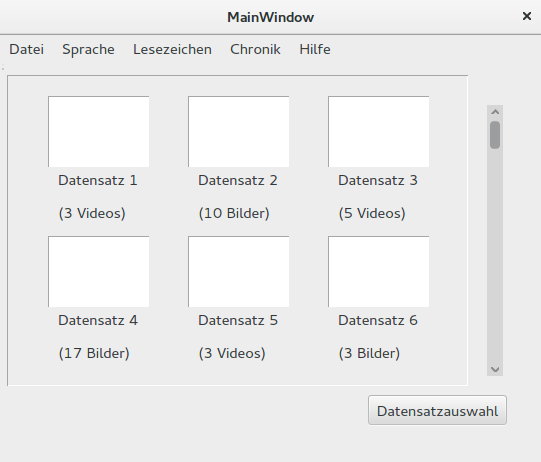
\includegraphics[width=1\linewidth]{img/Bibliothek}
Das erste Fenster beinhaltet die Bibliothek und außerdem ein Menü. In der Menüleiste kann im Punkt Datei ein neuer Datensatz ausgewählt oder das Programm beendet werden.  Unter Sprache kann die aktuelle Sprache ausgewählt werden. Unter Lesezeichen können Suchergebnisse geöffnet werden, die als Lesezeichen gespeichert wurden. In der Chronik kann ein Suchergebnis der letzten 5 Suchen geöffnet werden. Über den Menüpunkt Hilfe kann eine Anleitung oder ein About-Fenster geöffnet werden.
In der Bibliothek befinden sich die Datensätze aus dem Standardordner und zuletzt verwendete. Daraus kann ein Datensatz ausgewählt werden, in dem sich das Bild/Video befindet, nach dem gesucht werden soll. Mithilfe des Buttons 'neuer Datensatz' kann auch ein anderer Ordner als Datensatz gewählt werden.

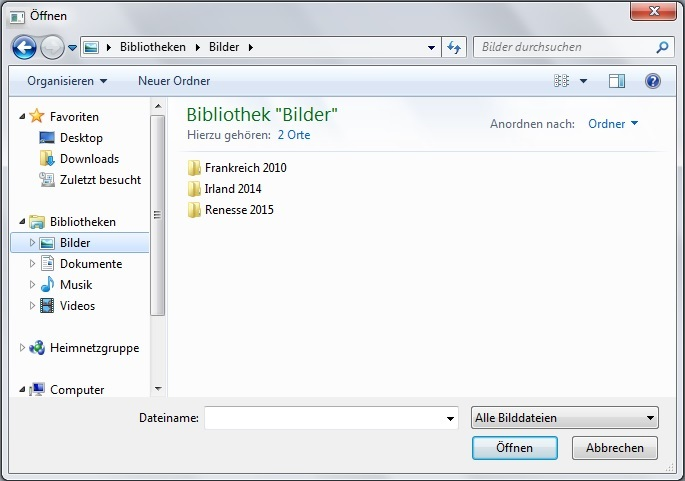
\includegraphics[width=1\linewidth]{img/FileChooser}
Hier kann der Benutzer einen Bild- oder Videodatensatz auswählen.

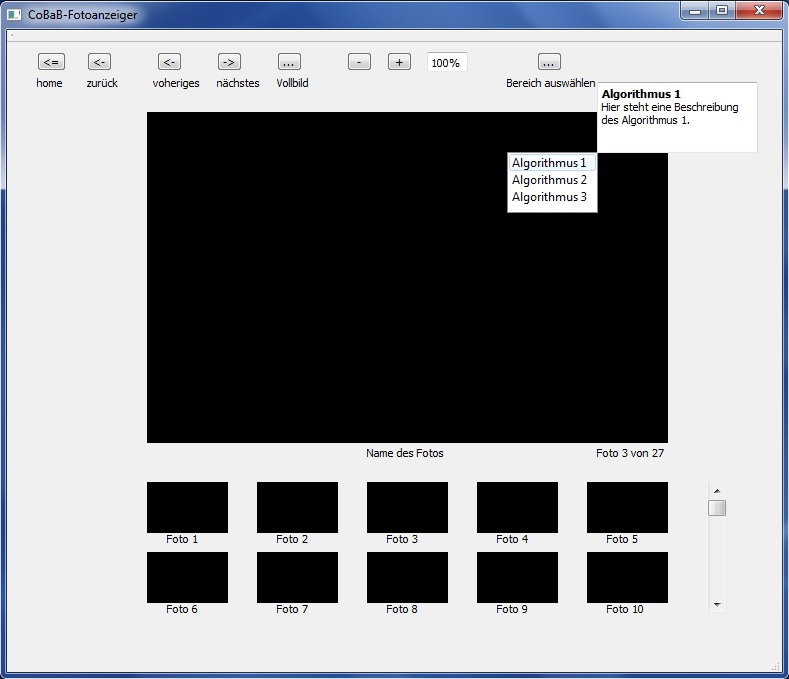
\includegraphics[width=1\linewidth]{img/Fotoanzeiger}
Über den 'Home' Button oben links kommt der Benutzer zurück zur Bibliothek. Beim Klicken des 'zurück' Buttons kann ein Schritt rückgängig gemacht werden, man kommt also zum vorherigen Fenster. Diese Buttons werden in den nächsten Fenstern immer an der gleichen Stelle sein.

Nach der Auswahl eines Datensatzes öffnet sich ein Bild-/Videoanzeiger, je nach dem, ob ein Bild- oder Videodatensatz gewählt wurde. Über die Buttons 'vorheriges' und 'nächstes' kann der Benutzer durch die Bilder/Videos browsen und ein geeignetes auswählen. Über den Button Vollbild kann das Bild/Video im Vollbildmodus angezeigt werden.
Bei einem Rechtsklick auf das Bild werden die Algorithmen aufgelistet, die für diese Suche zur Verfügung stehen. Fährt man mit der Maus über einen solchen Algorithmus, dann erscheint eine Beschreibung zu diesem.
In den Bildern werden außerdem, falls vorhanden, Annotationen angezeigt. Davon kann eine (mit Klick darauf) ausgewählt werden. Optional kann auch ein eigenes Rechteck gezogen werden. Mit Rechtsklick auf eine Annotation erscheint eine Auswahl aller Suchalgorithmen, die für diese Annotation in Frage kommen. Der Benutzer kann durch Klicken auf einen Algorithmusnamen mit dem Programm fortfahren.

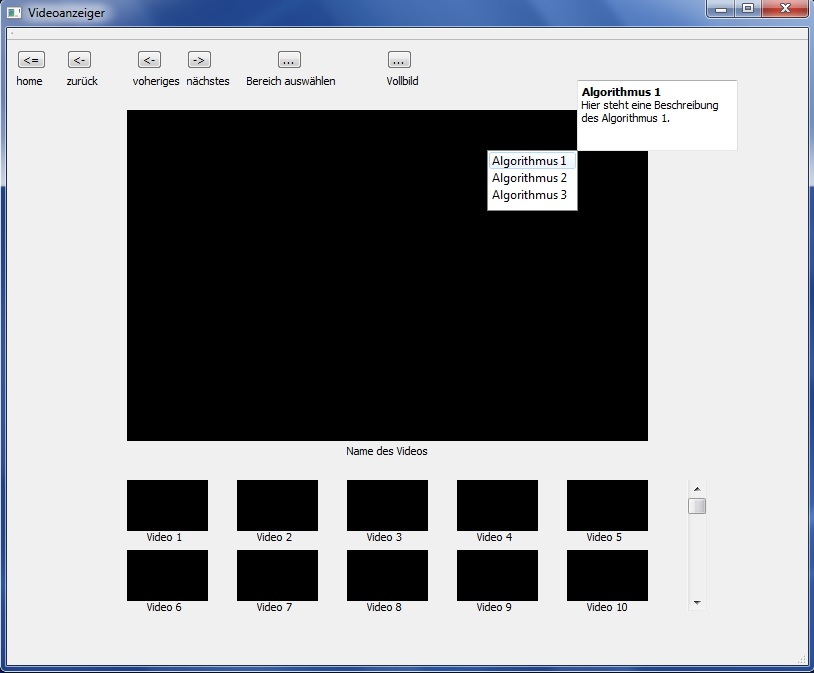
\includegraphics[width=1\linewidth]{img/Videoanzeiger}
Der Videoanzeiger bietet alle Funktionen des oben beschriebenen Fotoanzeigers. Zusätzlich können auch Videos abgespielt werden. Dabei wird im Player, ähnlich zu YouTube, Play, Pause, ein Fortschrittsbalken und die vergangene Zeit angezeigt. 

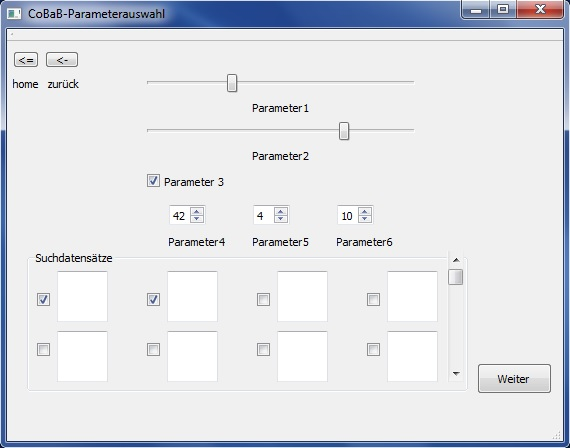
\includegraphics[width=1\linewidth]{img/Parameterauswahl}
Nach der Auswahl eines Suchverfahrens, kann man Parameter für den Suchalgorithmus festlegen. Außerdem können weitere Datensätze ausgewählt werden, in denen gesucht werden soll.

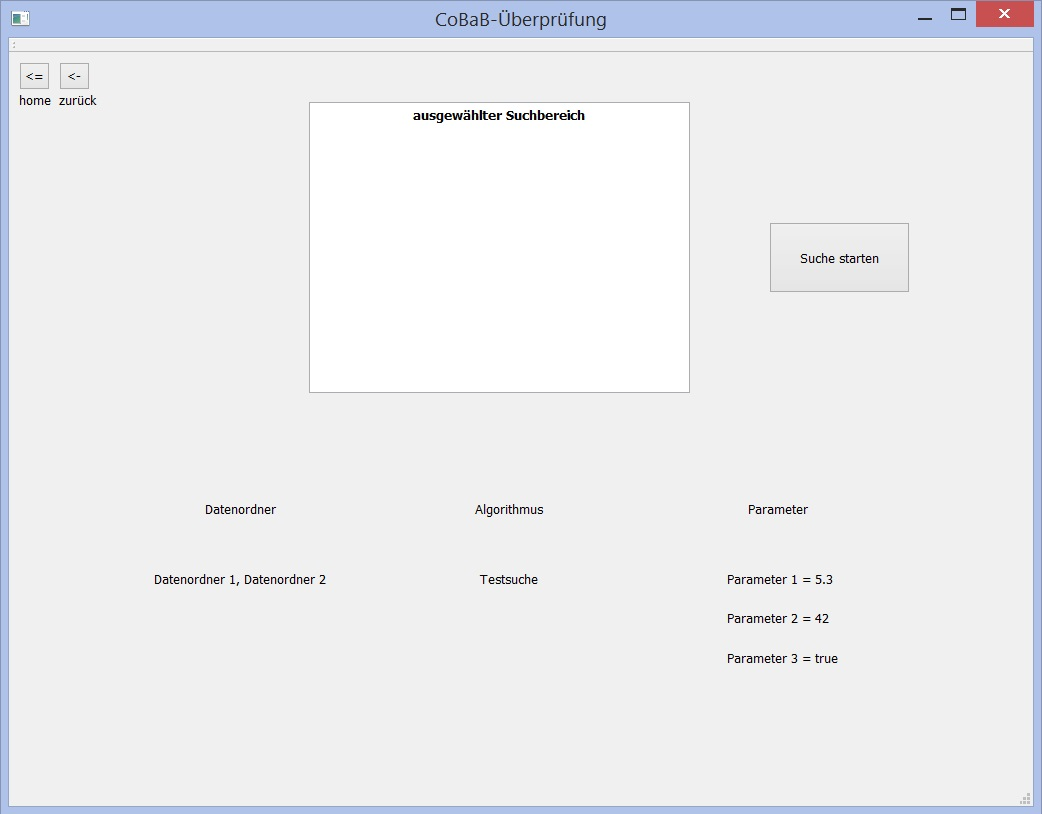
\includegraphics[width=1\linewidth]{img/Ueberpruefung}
Im Überprüfungsfenster wird noch einmal die aktuelle Auswahl angezeigt: der gewählte Bild-/Videoausschnitt, die Datensätze, in denen gesucht wird, der Suchalgorithmus und die Parameter. Wenn der Benutzer an diesen Werten nichts mehr ändern will, kann er nun über den Button 'Suche starten' das Suchverfahren mit der gezeigten Auswahl starten.

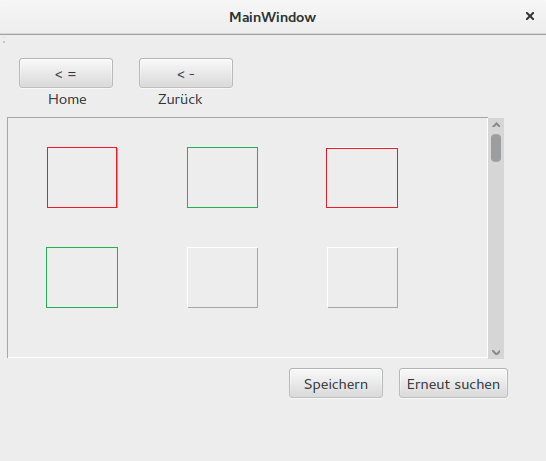
\includegraphics[width=1\linewidth]{img/Suchergebnisse}
Während der Suche wird eine Fortschrittsanimation in dem Fenster angezeigt, in dem dann die Suchergebnisse zu sehen sein werden. Wenn alle Ergebnisse angezeigt werden, kann das Suchergebnis über den Button als Lesezeichen gespeichert werden.\newline 
Der Benutzer kann durch einen Klick auf ein Bild dieses als positiv (grüner Kasten) bewerten. Durch einen weiteren Klick wird es negativ (roter Kasten) und durch noch einen Klick wieder neutral (kein Kasten) bewertet. Durch einen Klick auf den Button 'Erneut suchen', wird das Feedback an den Algorithmus übermittelt und eine neue verbesserte Suche gestartet.
\pagebreak

\section{Entwicklungsumgebung}
\subsection{Software}
\begin{itemize}
\item Sprache im Team
	\begin{itemize}[label={--}]
		\item Es wird auf Deutsch kommuniziert.
	\end{itemize}
\item Betriebssystem
	\begin{itemize}[label={--}]
		\item Die zum Entwickeln verwendete Betriebssysteme sind Windows 8, Fedora 22 und Ubuntu 14.
	\end{itemize}
\item Entwicklung
	\begin{itemize}[label={--}]
		\item Es wird auf C++ (Version 14) mit Standardbibliotheken programmiert
		\item Es wird mit Qt5.5 Bibliotheken gearbeitet. Als Tools werden QtDesigner und QtCreator verwendet.
	\end{itemize}
\item Versionsverwaltung
	\begin{itemize}[label={--}]
		\item Die Versionierung erfolgt mittels Git 1.9.1.
	\end{itemize}
\item Dokumentation
	\begin{itemize}[label={--}]
		\item Zum Aufbau von Phasendokumenten wird hauptsächlich LaTeX verwendet.
	\end{itemize}
\item Quelltext
	\begin{itemize}[label={--}]
		\item Quellcode und Kommentare werden auf Englisch verfasst.
		\item Es werden "C++ coding style conventions" verwendet.
		\item Die Dokumentation des Quelltextes erfolgt über Doxygen.
	\end{itemize}
\end{itemize}

\subsection{Hardware}
\begin{itemize}
	\item Es werden diverse Standardrechner mit Intel und AMD CPUs zum Aufbau des Programms benutzt.
\end{itemize}


\section{Glossar}
\printglossaries

\end{document}
